\documentclass[11pt]{article}
\usepackage{fancyhdr}
\usepackage[usenames, dvipsnames]{xcolor}
\usepackage{amsmath,amssymb,graphicx}
\newcommand{\HRule}{\rule{\linewidth}{0.5mm}}
\pagestyle{fancy}
\lfoot{\small \color{gray}Tom Peerdeman \& Ren\'e Aparicio Saez}
\cfoot{\thepage}
\rfoot{\small \color{gray}Studentnr: 10266186 \& 10214054}
\begin{document}
	\begin{titlepage}
	\begin{center}
		\textsc{\Large Besturingssystemen}\\[0.5cm]
		\HRule \\[0,4cm]
		\textsc{\huge \bfseries FAT-12 errors}
		\HRule \\[2cm]
		\begin{minipage}{0.4\textwidth}
			\begin{flushleft}\large
				\emph{Auteurs: Tom Peerdeman \& Ren\'e Aparicio Saez}\\
			\end{flushleft}
		\end{minipage}
		\begin{minipage}{0.4\textwidth}
			\begin{flushright}\large
			\emph{Datum: 25-05-2012\\\'}\\
			\end{flushright}
		\end{minipage}
	\end{center}
	\end{titlepage}


	\begin{center}
		\textbf{\underline{\large Opgave 4: Beschadigingen in een FAT-12 localiseren}}
	\end{center}
	\textbf{Inleiding}\\
	Een FAT (File Allocation Table) is een single linked list. Deze bevat 'entries' voor clusters. Iedere entry geeft aan waar de volgende cluster gevonden kan worden. Of, als er geen nieuwe clusters meer zijn, dat alle clusters opgehaald zijn. Deze clusters samen vormen een file. Dit is een eenvoudige en betrouwbare manier om files op te slaan. Echter kunnen er wel fouten optreden in de FAT. Specifiek wordt er gekeken naar de 12 bits variant, FAT-12.
	\begin{figure}[h]
		\begin{center}
		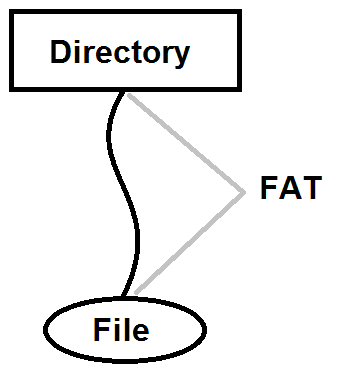
\includegraphics[width=0.4\textwidth]{fatgoed.png}
		\caption{Schematische weergave van de werking van een 	FAT}
		\end{center}
	\end{figure}
	\newpage
	\textbf{Fouten overzicht}\\
	Er zijn verschillende soorten fouten die kunnen optreden in een FAT-12. Sommige fouten zijn eenvoudig op te lossen en op te sporen.\\\\
	Mogelijke fouten in de FAT zijn bijvoorbeeld:
	\begin{itemize}
		\item Loops in de FAT
		\begin{itemize}
			\item Meerdere verwijzingen 
		\end{itemize}
		\item Dubbel gebruik van een deel van de FAT
		\item Twee dezelfde files in \'e\'en directory
		\item Twee dezelfde files in verschillende directory's
		\item Incorrect eindigende link
		\item Een bestand komt nog voor in de FAT maar staat niet meer in de directory
		\item Een bestand dat bestaat in de directory maar niet in de FAT
	\end{itemize}
	


\end{document}
